% Copyright 2023 Louis Paternault
%
% This work may be distributed and/or modified under the following licences.
%
% LaTeX Project Public Licence
% ----------------------------
%
% This work may be distributed and/or modified under the
% conditions of the LaTeX Project Public License, either version 1.3
% of this license or (at your option) any later version.
% The latest version of this license is in
%   http://www.latex-project.org/lppl.txt
% and version 1.3 or later is part of all distributions of LaTeX
% version 2005/12/01 or later.
%
% Creative Commons by-sa 4.0
% --------------------------
%
% This work may be distributed and/or modified under the
% conditions of the Creative Commons Attribution-ShareAlike 4.0 International
% (CC BY-SA 4.0). The full text of this license is in
% https://creativecommons.org/licenses/by-sa/4.0/

% Compile using LuaLaTeX
%$ lualatex $basename

\documentclass[tikz]{standalone}

\usepackage{siunitx}

\begin{document}
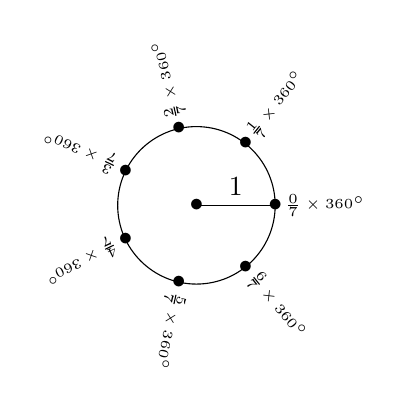
\begin{tikzpicture}
  \draw (0, 0) circle (1);
  \draw (0, 0) node{$\bullet$} -- (0:1) node[midway, above]{$1$};
  \foreach \i in {0, ..., 6}{
    \draw ({\i*360/7}:1) node{$\bullet$};
    \draw ({\i*360/7}:1) node[anchor=west, rotate={\i*360/7}]{\tiny $\frac{\i}{7}\times\ang{360}$};
  }
\end{tikzpicture}

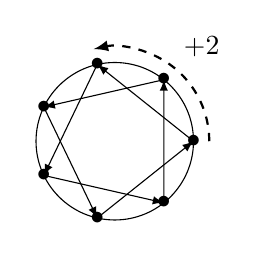
\begin{tikzpicture}[scale=1]
  \draw (0, 0) circle (1);
  \foreach \i in {0, ..., 6}{
    \draw[-latex] ({\i*360/7}:1) -- ({(\i+2)*360/7}:1) node{$\bullet$};
  }
  \draw[-latex, dashed, thick] (0:1.2) arc[start angle=0, delta angle={2*360/7}, radius=1.2] node[midway, above right]{$+2$};
\end{tikzpicture}

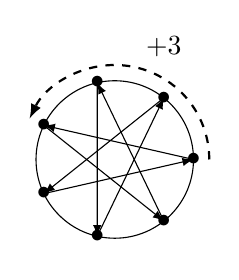
\begin{tikzpicture}[scale=1]
  \draw (0, 0) circle (1);
  \foreach \i in {0, ..., 6}{
    \draw[-latex] ({\i*360/7}:1) -- ({(\i+3)*360/7}:1) node{$\bullet$};
  }
  \draw[-latex, dashed, thick] (0:1.2) arc[start angle=0, delta angle={3*360/7}, radius=1.2] node[midway, above right]{$+3$};
\end{tikzpicture}

\end{document}
